\documentclass[11pt]{article}
\usepackage{natbib}
\usepackage{array}
\usepackage{graphicx}
\graphicspath{ {images/} }
\begin{document}

\title{Learning to Solve Arithmetic Word Problems Using Sentence Simplification}
\author{
	Vishal Rajpal\\
	Northeastern University\\
	rajpal.vi@husky.neu.edu\\
}
\date{}
\maketitle

\begin{abstract}
In order to respond to an arithmetic word problem correctly one needs to understand the question to an extent which allows determining the constraints. These are mostly semantic and are imposed by the question on its answer. Constraints from individual sentences suggest a mathematical operation and when the operators from these sentences are used collectively the answer can be derived. To extract the constraints efficiently, a concept of Syntactic Pattern is introduced which is generated by parsing the sentence using a dependency parser. It encapsulates all the relevant information in a sentence including the subject, verb and object with its quantity. Another important method for this thesis which relies on syntactic patterns is Sentence Simplification. The idea is to have a subject, verb, an object and other necessary parts of speech in the sentence so that it suggests a single operation. Based on the identified patterns a sentence may be simplified to multiple sentences. This would make the classification process easier since the sentences are less complex. To this end, it would be the classifier's job to classify the sentence to a mathematical operator. The identified operators for individual sentences are used to build a mathematical equation for the entire word problem. The results based on 3 datasets are reported and seem promising as compared to the existing systems.
\end{abstract}

\section{Introduction}
Answering arithmetic word problems has gained a lot of interest in recent years. The problem is attractive to NLP since the text is concise and relatively straightforward with identifiable semantic constraints. As these problems are directed towards elementary school students, they begin by describing a partial world state, followed by simple quantified updates or elaborations and end with a quantitative question. This information can be mapped to basic operations(addition, subtraction, multiplication and division) and an equation can be created corresponding to the problem text. 

There have been a number of attempts to solve arithmetic word problems through Machine Learning. 
All the approaches which are not template based \citep{ARIS}, \citep{RoyTACL15} and \citep{RoyR15} use different methods to extract similar information. Based on different ways the information is represented, an equation is built for the problem text. The template based method of \citep{Kushman} implicitly assumes that the solution will be generated from a set of predefined equation templates. Some of these methods only solve addition and subtraction problems \citep{ARIS}, \citep{RoyTACL15} while \citep{RoyR15} and \citep{Kushman} can solve problems for all operations.

The approach presented in this thesis can solve a general class of addition and subtraction arithmetic word problems without any predefined equation templates. In particular, it can handle an arithmetic problem as shown in Table 1.

\begin{table}[h!]
\centering
\begin{tabular}{ | m{25em} | }
\hline
Example 1:\\
\hline
For Halloween, Debby and her sister combined the candy they received. Debby had 32 pieces of candy while her sister had 42. If they ate 35 pieces the first night, how many pieces do they have left?\\
\hline
\end{tabular}
\caption{Example Arithmetic Word Problem.}
\label{table:1}
\end{table}

To derive the solution to this problem, the approach needs to understand that \textit{they} refers to \textit{Debby and her sister}. Hence, the number of candies need to be summed up and then \textit{35 candies} need to be subtracted from the total number of candies. 

While a solution to these problems requires extracting information and composing numeric expressions, if the sentence is too complex it is hard to extract information accurately.

At the heart of the technical approach, the novel notion of \textit{Sentence Simplification} is involved. Once the sentences in the problem text are simplified, extracting information becomes easier. Each sentence in the problem is simplified to a level where it consists information which is able to be mapped to a single operator. This allows us to decompose the entire problem to a collection of simplified sentences as operator prediction problems. Each sentence represents the quantitative information with the mapped operator. These predictions(operators with the quantitative information) can be combined together to form a mathematical equation.

The approach focuses on addition and subtraction problems currently, but learning to classify operators will allow us to generalize the approach to multiplication and division problems as well. In particular, the system was able to solve Example 1 although it had never seen the problem before and required both addition and subtraction operations.

The approach is evaluated on 3 datasets, achieving competitive performance on all of them. The next section describes the related work in the area of automated arithmetic word problem solving. The theory of sentence simplification is then presented. Later the information decomposition strategy that is based on it is discussed. Section 4 presents the overall computational approach, including the way classifier learns to classify simplified sentences to operators. Finally, experimental study is discussed followed with a conclusion.

\section{Related Work}
Most of the previous work in automated arithmetic problem solvers has focused on a restricted subset of problems.The approach described in \citep{RoyTACL15} handles problems with all basic operations but makes assumptions about the number of quantities in the problem text and the number of steps required to solve the problem. In contrast, our approach does not make any assumptions about the data in the problem text. Kushman's approach \citep{Kushman} tries to map numbers from the problem text to predefined equation templates and implicitly assume that similar equation forms have been seen in the training data. On the contrary, our system does not rely on pre-defined templates and hence is able to solve questions of type which have never been seen before.  The approach described in \citep{ARIS} might be the most related to ours. It handles addition and subtraction problems and tries to predict an operator for the verb in the problem text. Hence, it requires additional annotated data for verb categories. Our approach uses the information of the verb present in the sentence and handles addition and subtraction problems for now, but there is no requirement of additional annotated data. Refer to Section 5 for how the information from verbs is used as a feature. 

Most of the methods mentioned above are able to solve problems with all basic operations but our approach is easily generalizable to all the operators and also it performs competitevely compared to all other approaches. 

\section{Arithmetic Problem Representation}

Our approach addresses word problems that include addition and subtraction operations. Given a problem text, multiple fragments are extracted from it  where each fragment is a simplified version of the information presented in the sentence. We refer to these fragments as simplified sentences. Each fragment is represented based on the Parts of Speech it contains. Below are the parts of speech we consider in our representation:


\textbf{Adjective:} A problem text might have multiple types of same entities. Consider the below example:

 \begin{table}[h!]
\centering
\begin{tabular}{ | m{25em} | }
\hline
 \textbf{A pet store had 13 siamese cats and 5 house cats.}\\
\hline
 siamese cats\\
\hline
house cats.\\
\hline
\end{tabular}
\caption{Entities with Adjective.}
\label{table:2}
\end{table}

Though the example sentence has cats as the noun, but based on the adjectives\textit{(siamese and house)} there were siamese cats and house cats.
\vspace{4mm}

\textbf{Cardinal:} Cardinals are the numbers present in the problem text. We associate them to nouns based on the index at which they occur. Mostly, they occur before the noun and hence associating it is not difficult. Sometimes, the cardinal is a reference to an already occured noun. Consider the example below:

\begin{table}[h!]
\centering
\begin{tabular}{ | m{25em} | }
\hline
\textbf{He bought 2 games from a friend and bought 5 more at a garage sale.}\\
\hline
2 games\\
\hline
5 games\\
\hline
\end{tabular}
\caption{Entity with Cardinal Numbers.}
\label{table:3}
\end{table}

\textit{5 more} in the above example refers to games. We associate this to the last quantified noun encountered in the sentence.
\vspace{4mm}

\textbf{Conjunction:} Conjunctions are stored mainly to simplify the sentence. Most importantly, the index at which it occurs in the sentence plays a crucial role in creating simplified sentences.
\vspace{4mm}

\textbf{Determiner:} Determiner by definition is \textit{a modifying word that determines the kind of reference a noun or a noun group has.} 

\begin{table}[h!]
\centering
\begin{tabular}{ | m{25em} | }
\hline
\textbf{There are 28 students and every student has their own lunchbox.}\\
\hline
\textit{Every} is a determiner\\
\hline
\end{tabular}
\caption{Sentence with Determiner.}
\label{table:4}
\end{table}

In the above example, \textit{Every} is a determiner and when considering it, our system will be able to extract the information that there are \textit{28 lunchboxes}.
\vspace{4mm}

\textbf{Existential/Expletive:} Since, existentials indicate the existence or presence of something, they are an important part of speech for our system. Also, when the sentences are simplified, the existentials are added to the fragments which don't have them. Refer to the next section for more details.

\begin{table}[h!]
\centering
\begin{tabular}{ | m{25em} | }
\hline
\textbf{There are 11 rulers and 34 crayons in the drawer.}\\
\hline
There are 11 rulers in the drawer.\\
\hline
There are 34 crayons in the drawer.\\
\hline
\end{tabular}
\caption{Simplified sentences based on Existential.}
\label{table:5}
\end{table}

After the split based on conjunction \textit{and} the expletive \textit{There} is added to the fragment after the conjunction.
\vspace{4mm}

\textbf{Noun:} Nouns are important for answering the arithmetic word problems. Each problem text has some nouns in form of a subject \textit{(acting entity)} or an object \textit{(Entity that is acted upon by the subject)}. All the nouns are extracted from the simplified sentence and stored as a list. 
\vspace{4mm}

\textbf{Preposition:} Prepositions are helpful to keep track of location or time. Also, when simplifying sentences based on conjunctions we add prepositions to the fragments which are missing them. Refer to the next section for more details and example.
\vspace{4mm}

\textbf{Verb:} Verbs are important for out system to predict the type of action taken by the subject. Determining the kind of action helps to predict an operation. More details on this in Section Features.
\vspace{4mm}

\textbf{WHAdverb:} Existence of a WHAdverb mostly indicates the beginning of a question. Hence, having the WHAdverb in our representation helps us in the classification process. Refer to the Section Features.

\section{Sentence Simplification and Problem Decomposition}
Sentences in an arithmetic word problem are sometimes complex. Hence, it is difficult to extract information from such sentences. Even more challenging is to predict the impact of the sentence on the result. 

\begin{table}[h!]
\centering
\begin{tabular}{ | m{25em} | }
\hline
Example 2:\\
\hline
Henry had 11 dollars. For his birthday he got 18 more dollars but spent 10 on a new game. How much money does he have now?\\
\hline
\end{tabular}
\caption{Example Arithmetic Word Problem.}
\label{table:6}
\end{table}

The second sentence in the above example is complex for a machine learning algorithm. It has addition and subtraction operation in a single sentence. Our idea is to simplify the sentence to multiple simple sentences so that each simplified sentence has a single operation. Below are the simplified sentences for the second sentence in the above example:

\begin{table}[h!]
\centering
\begin{tabular}{ | m{25em} | }
\hline
 \textbf{For his birthday he got 18 more dollars but spent 10 on a new game.}\\
\hline
 For his birthday he got 18 more dollars.\\
\hline
He spent 10 dollars on a new game.\\
\hline
\end{tabular}
\caption{Simplified Sentences.}
\label{table:7}
\end{table}

We create a mapping for each sentence in the problem text to its simplified sentences by extracting their relational dependencies for each sentence from the stanford dependency parser\footnote{http://stanfordnlp.github.io/CoreNLP/ }. Currenly, our simplification system simplifies sentences based on conjunctions and commas. There are certain rules when simplifying the sentence.

\subsection{Rules for simplifying sentences based on conjunctions.}
 When a conjunction is encountered, our simplification system attempts to create two simplified sentences from the actual sentence. The first sentence is the part before the conjunction while the second sentence is the part after the conjunction.

But, after the split there may be some words which would be required in the second sentence. Consider the example in Table 4:

\begin{table}[h!]
\centering
\begin{tabular}{ | m{25em} | }
\hline
 \textbf{Example Sentence.}\\
\hline
The school cafeteria ordered 42 red apples and 7 green apples for students lunches.\\
\hline
\end{tabular}
\label{table:8}
\end{table}

In the sentence above, the split based on conjunction \textit{and} will result in the first sentence with a subject while the second will not have a subject and a verb. Hence, there are some rules for adding words to the second simplified sentence.

\subsubsection{Rules for adding words to second simplified sentence.}
\begin{enumerate}
 \item 
If the first sentence starts with an existential and the second does not, add the existential to the second sentence as well.

\item 
If the first sentence starts with an existential and has a verb after it, If the second sentence does not have either expletive or verb, add them to the second sentence. Consider the below example:

\begin{table}[h!]
\centering
\begin{tabular}{ | m{25em} | }
\hline
 \textbf{There were 2 siamese cats and 4 house cats.}\\
\hline
There were 2 siamese cats.\\
\hline
There were 2 house cats.\\
\hline
\end{tabular}
\caption{Example sentence for this rule.}
\label{table:9}
\end{table}

The expletive and verb were added to second sentence based on the simplification rule mentioned above.

\item
If the first sentence starts with a noun, and if the second sentence starts with a verb, the noun from the first sentence will be added to the second.

\begin{table}[h!]
\centering
\begin{tabular}{ | m{25em} | }
\hline
 \textbf{Joan ate 2 oranges and threw 3 apples.}\\
\hline
Joan ate 2 oranges.\\
\hline
Joan threw 3 apples.\\
\hline
\end{tabular}
\caption{Example sentence for this rule.}
\label{table:10}
\end{table}

\item 
If the first sentence starts with a noun and the second sentence has a \textit{noun verb} pattern, do nothing.

\begin{table}[h!]
\centering
\begin{tabular}{ | m{25em} | }
\hline
 \textbf{Tom has 9 yellow balloons and Sara has 8 yellow balloons.}\\
\hline
Tom has 9 yellow balloons.\\
\hline
Sara has 8 yellow balloons.\\
\hline
\end{tabular}
\caption{Example sentence for this rule.}
\label{table:11}
\end{table}

No words from the first sentence were added to the second since the second sentence had the \textit{noun verb (Sara has)} pattern.

\item
If the second sentence contains a preposition at the end and the first sentence does not have a preposition, the preposition from the second sentence will be added to the first. Consider the below example:

\begin{table}[h!]
\centering
\begin{tabular}{ | m{25em} | }
\hline
 \textbf{Joan found 6 seashells and Jessica found 8 seashells on the beach.}\\
\hline
Joan found 6 seashells on the beach.\\
\hline
Jessica found 8 seashells on the beach .\\
\hline
\end{tabular}
\caption{Example sentence for this rule.}
\label{table:12}
\end{table}

After splitting the sentence based on \textit{and} the preposition and the words after it \textit{on the beach} were added to the first sentence.

\item
Based on the output by the dependency parser and our rules, there might be some words which might not have been identified. But we still need those words in the simplified sentences.

\item
Therefore, the sentence simplification system identifies all the words which were not identified by our process. The words which appear before the conjunction are added to the first sentence at the right index. If the words appear after the conjunction, they are added to the second sentence.

\begin{table}[h!]
\centering
\begin{tabular}{ | m{25em} | }
\hline
 \textbf{He went to the orchard and picked peaches to stock up .}\\
\hline
Tom has 9 yellow balloons.\\
\hline
Sara has 8 yellow balloons.\\
\hline
\end{tabular}
\caption{Example sentence for this rule.}
\label{table:13}
\end{table}

\end{enumerate}

\subsection{Syntactic Pattern}
In this thesis, a new concept known as Syntactic Pattern is introduced which is basically a summarized information about a fragment. It is a pattern consisting of the initials of the parts of speech which appear in the fragment. The initials are arranged in the order in which the words appear in the sentence. Consider the below figure:

\begin{figure}[h!]
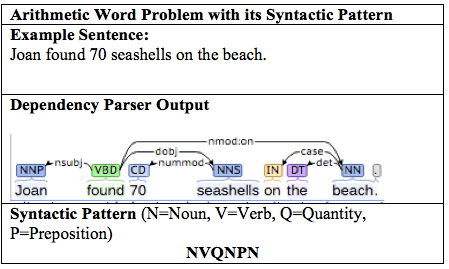
\includegraphics[width=1.0\textwidth]{Figure1}
\centering
\caption{\label{fig:Figure1}Example sentence of a word problem and its syntactic pattern.}
\end{figure}


\newpage
\bibliographystyle{apalike}
\bibliography{Thesis}



\end{document}